
As mentioned in Chapter 1, this research focuses on the strategic deployment of electric vehicle charging stations (EVCS) in urban environments. This chapter presents the experimental design, implementation, and analysis of a multi-objective optimization problem (MOOP) to solve the Electric Vehicle Charging Stations problem using the non-dominated genetic sorting algorithm II (NSGA-II). The goal is to optimize the locations and configuration of EVCS.

The problem is modeled with four conflicting objectives: (1) maximizing coverage , (2) maximizing charger speed, (3) minimizing the number of stations, and (4) minimizing the total number of chargers per station. These objectives often conflict with one another; for example, increasing coverage and charger speed usually requires deploying more chargers and stations, which conflicts with the goal of minimizing infrastructure.

NSGA-II was chosen for its proven effectiveness in tackling complex, multi-objective, nonlinear optimization problems with discrete decision variables. This algorithm is well suited for problems that require a variety of balanced solutions for decision-making.

\section{Experimental Environment}

The algorithm was implemented using the DEAP framework in Python. Experiments were run on a system with the following specifications:

\begin{itemize}
    \item OS: Windows 10
    \item Processor: Intel(R) Core(TM) i7-10610U CPU @ 1.80GHz   2.30 GHz
    \item RAM: 32 GB
    \item Python Version: 3.10
    \item Libraries: NumPy, DEAP, Matplotlib, Pandas
\end{itemize}

The demand data used is extracted from publicly available electric vehicle charging station data models, ensuring realistic modeling of public coverage needs.



\section{Dataset}
\subsection{Stations dataset}
In this research on electric vehicle charging stations (EVCS), we selected a California data set due to its leading role in the adoption of electric vehicles and the development of its charging infrastructure. In addition, the installation costs for the chargers were sourced from standard prices used across the United States.

California is among the regions that have implemented EV policies to reduce pollution. Furthermore, California boasts a high population density and a large number of electric vehicles and EV charging stations, providing a rich source of data on usage, location, and other key factors influencing the development of charging stations. This data enhances the potential for EV charging stations to be deployed in other regions.

In this experiment, we evaluate the performance of the NSGA-II algorithm. The test case is based on one of the California dataset, with the following details:


\begin{itemize}
    \item 100 potential locations for charging stations, each location has number of charger, with 1000 EVs in the area. The dataset includes the following attributes for each location:
    \begin{itemize}
        \item \textbf{Id}: charging station number.
        \item \textbf{Coordinates}: The geographical coordinates of each charging station location.
        \item \textbf{Charger speed (kW)}: The chargers speed power for each charger, (11.5, 14.2, 19.2, 25, 60, 62, 80, 120, 150, 180, 200, 240, 250, 300, 325, 350, 400).
        \item \textbf{Chargers per station}: The number of chargers installed at each station.
    \end{itemize}
\end{itemize}


\subsection{station cost dataset}
\begin{table}[h!]
    \centering
    \small % Reduce the font size for the table
    \begin{tabular}{|>{\raggedright\arraybackslash}p{2cm}|>{\raggedright\arraybackslash}p{3cm}|>{\raggedright\arraybackslash}p{2cm}|>{\raggedright\arraybackslash}p{2cm}|>{\raggedright\arraybackslash}p{3cm}|}
    \hline
    \textbf{Power Range} & \textbf{Type of Charger} & \textbf{Hardware Cost} & \textbf{Installation Cost} & \textbf{Total Estimated Cost} \\
    \hline
    3 kW - 7 kW & Level 1 or Level 2 Charger & \$500 - \$1,500 & \$300 - \$500 & \$800 - \$2,000 \\
    \hline
    7 kW - 22 kW & Level 2 Charger & \$1,500 - \$5,000 & \$1,000 - \$2,500 & \$2,500 - \$7,500 \\
    \hline
    50 kW - 100 kW & DC Fast Charger & \$30,000 - \$50,000 & \$50,000 - \$100,000 & \$80,000 - \$150,000 \\
    \hline
    100 kW - 150 kW & DC Fast Charger & \$50,000 - \$70,000 & \$50,000 - \$100,000 & \$100,000 - \$170,000 \\
    \hline
    150 kW - 200 kW & DC Fast Charger & \$70,000 - \$100,000 & \$100,000 - \$150,000 & \$170,000 - \$250,000 \\
    \hline
    200 kW - 350 kW & Ultra-Fast Charger & \$100,000 - \$150,000 & \$150,000 - \$250,000 & \$250,000 - \$400,000 \\
    \hline
    350 kW - 400 kW & Ultra-Fast Charger & \$120,000 - \$150,000 & \$150,000 - \$250,000 & \$270,000 - \$400,000 \\
    \hline
    \end{tabular}
    \caption{Cost Estimates for Different Types of EV Chargers}
    \end{table}




\subsection{Decision Variables}

The optimization problem considers a set of locations (stations), where each station can use a number of electric vehicle chargers (EVCs) with a specified charging speed. The decision variables include:

\begin{itemize}
    \item $x_i \in \{0,1\}$: Binary variable indicating whether a station is deployed at location $i$.
    \item $c_i \in \{0, 1, 2, ..., C_{max}\}$: Integer variable indicating the number of chargers at location $i$.
    \item $c_i \in \{0, 1, 2, ..., C_{max}\}$: Integer variable indicating the number of station $i$.
    \item $s_i \in \{s_1, s_2, ..., s_k\}$: Discrete variable indicating the speed of chargers at Station $i$.
\end{itemize}

\subsection{Objective Functions}

\begin{enumerate}
    \item \textbf{Maximize Coverage ($f_1$)}: Coverage is defined as the percentage of demand points (e.g., traffic or residential clusters) that fall within the effective range of any installed station. 
    \[
    f_1 = \frac{\sum_{j=1}^{m} \delta_j}{m}, \quad \delta_j = \begin{cases}
    1 & \text{if demand point } j \text{ is covered by any station} \\
    0 & \text{otherwise}
    \end{cases}
    \]

    \item \textbf{Maximize Charger Speed ($f_2$)}: Charger speed is value of the installed charger speed, where higher-speed chargers receive a higher weight.
    \[
    f_2 = \frac{\sum_{i=1}^{n} x_i \cdot c_i \cdot s_i}{\sum_{i=1}^{n} x_i \cdot c_i}
    \]

    \item \textbf{Minimize Number of Stations ($f_3$)}:
    \[
    f_3 = \sum_{i=1}^{n} x_i
    \]

    \item \textbf{Minimize Number of Chargers ($f_4$)}:
    \[
    f_4 = \sum_{i=1}^{n} c_i
    \]
\end{enumerate}


\subsection{Constraints}

The optimization is subject to the following constraints:

\begin{itemize}
    \item \textbf{Budget Constraint}:
    \[
    \sum_{i=1}^{n} \left(x_i \cdot F + c_i \cdot V(s_i)\right) \leq B
    \]
    where $F$ is the cost per station, $V(s_i)$ is the cost of a charger with speed $s_i$, and $B$ is the total budget.
    
    \item \textbf{Location Feasibility}: Only pre-approved location can be selected, based on land availability and zoning regulations.

    \item \textbf{Station Capacity }: Each station has a maximum number of chargers it can accommodate.

    \item \textbf{Redundancy Constraint}: Ensure no  stations are placed without covering demand.
\end{itemize}



\section{NSGA-II Algorithm Setup}

\subsection{Overview}

As discussed in Chapter 3, NSGA-II is an evolutionary algorithm that maintains a population of candidate solutions. In each generation, new offspring are generated through crossover and mutation. The next generation is then selected based on Pareto dominance and a crowding distance metric, which together promote both optimality and diversity within the population.

\subsection{Parameters}

\begin{itemize}
    \item Population Size: 100
    \item Number of Generations: 50
    \item $\mu$ (Number of Individuals Selected for the Next Generation): 50
    \item $\lambda$ (Number of Offspring Generated Each Generation): 100
    \item Crossover Probability ($cxpb$): 0.7
    \item Mutation Probability ($mutpb$): 0.2
    \item Selection Method: NSGA-II (Non-dominated Sorting Genetic Algorithm II)
    \item Crossover Operator: Two-Point Crossover
    \item Mutation Operator: Shuffle Index Mutation
    \item Possible power speed : [11.5, 14.2, 19.2, 25, 60, 62, 80, 120, 150, 180, 200, 240, 250, 300, 325, 350, 400]
    \item The dataset is described in the Dataset section(Stations dataset).

\end{itemize}

\subsection{Encoding Strategy}

Each individual in the population is encoded as a tuple:

\[
\textbf{Chromosome} = \left[ (x_1, c_1, s_1), (x_2, c_2, s_2), ..., (x_n, c_n, s_n) \right]
\]

This representation allows flexible adjustment of whether a station is deployed, how many chargers it has, and their speed types.

\subsection{Steps of the Applied NSGA-II Algorithm}
\subsubsection*{Step 1: Preprocessing the Data}

In this experiment, The stations data was imported using the OpenChargeMap API~\cite{openchargemap} through the \texttt{openchargemap} fetcher. The data was filtered to include only stations from the United States ("country code": "US") and from California ("state": "California")As mentioned in the dataset section. After filtering, we selected the important columns for this expierenment, which were: ``station\_id'', ``latitude'', ``longitude'', ``number\_of\_points'', and ``power\_kw''. We then converted the ``number\_of\_points'' and ``power\_kw'' columns into numeric values so that they could be processed correctly during optimization process. Some column names have been updated to make the data more easier. 

In addition, since one of our objectives relates to coverage, it was necessary to calculate the coverage for each selected station. To achieve this, we implemented the \texttt{calculate\_coverage} method. This method computes the total coverage based on the distances between stations. We then used the \texttt{add\_coverage} method to assign these calculated coverage values to the stations dataset.

In the end, As shown in Figure~\ref{fig:Stations Dataset}the data was cleaned, formatted,to use as input of the NSGA-II algorithm used in this study. 
\newline
\begin{figure}[h]
    \centering
    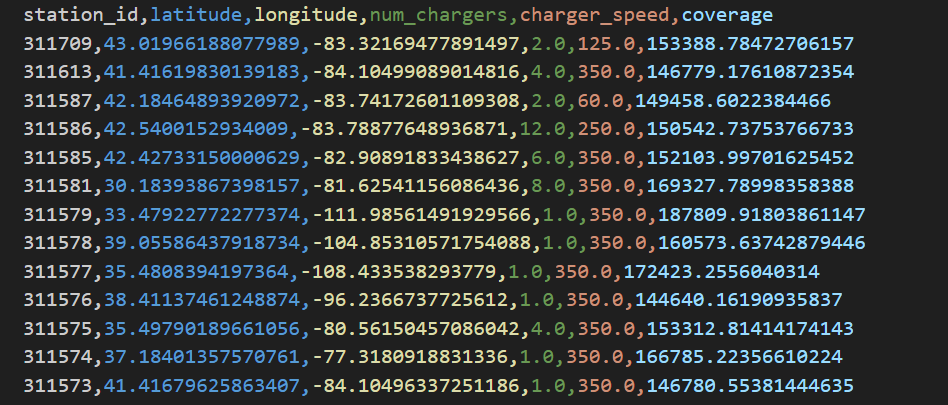
\includegraphics[width=\textwidth]{../Figures/stations_with_coverage.PNG}
    \caption{Stations Dataset}
    \label{fig:Stations Dataset}
\end{figure}
\newline
\subsubsection*{Step 2: Define the Multi-Objective Optimization Problem} 
In this step, the electric vehicle charging station (EVCS) problem was defined as a multi-objective optimization problem with four conflicting goals. These objectives are: (1) maximizing geographical coverage, ensuring that as many areas as possible are served by at least one station; (2) maximizing charger speed, which helps reduce the waiting time for electric vehicle (EV) users; (3) minimizing the number of installed charging stations, which contributes to reducing the overall infrastructure cost; and (4) minimizing the total number of chargers across all selected stations to further manage costs and operational complexity.

To implement this formulation, we used the DEAP framework\cite{Fortin2012}. The problem was modeled using a custom fitness class where the objectives were assigned specific weights: positive weights (1.0) for maximizing coverage, positive weights (1.0) for maximizing charger speed, negative weights (-1.0) for minimizing the number of stations and negative weights (-1.0) for minimizing the number of chargers. This formulation allows the algorithm to simultaneously balance service quality and cost efficiency. Each individual in the population represents a unique combination of selected charging stations, and the fitness evaluation returns values to each of the four objectives. 


\subsubsection*{Step 2: Define, and initialize DEAP Components}

In this step, the DEAP framework is utilized to define the requirement components for the evolutionary algorithm, such as the fitness function, individual structure, and algorithm settings. These settings include population size, selection strategy, and the methods for crossover and mutation. To initialize these components, we first create a toolbox using DEAP's base.Toolbox. The toolbox is then populated with several registered functions that define the operations for the evolutionary process.

In additon, the individual function is registered to generate an individual from a specified structure using the tools.initIterate method. The population function initializes the population by creating multiple individuals through tools.initRepeat. The mate function, which controls the crossover operation, is defined with the cxTwoPointCheck method. Similarly, the mutation operation is defined using mutShuffleIndexesCheck with a mutation probability. For selection, the selNSGA2 method is registered, which ensures that the selection process follows the NSGA-II strategy for multi-objective optimization. 

Howerver, the evaluate function is linked to the toolbox to evaluate individuals based on their fitness values.

By registering these functions, the necessary components of the evolutionary process are prepared, allowing the algorithm to run efficiently.


\subsubsection*{Step 3: Define Objective Functions}
In this step, we define the four objective functions, as mentioned in the 'Objective Functions' subsection above, which will guide the evolutionary algorithm towards finding the best solution:

\begin{itemize}
    \item \textbf{Objective 1: Maximize Coverage} \\
    The \texttt{calculate the coverage} function. This function calculates the total coverage between stations by calculating the distance between them. 

    \begin{equation}
    \text{Coverage} = \sum_{i=1}^{n-1} \sum_{j=i+1}^{n} d(s_i, s_j)
    \end{equation}

    \noindent
    Where:
    \begin{itemize}
        \item $n$ is the total number of selected stations,
        \item $s_i$ and $s_j$ are the coordinates (latitude and longitude) of the selected station,
        \item $d(s_i, s_j)$ is the geographical distance between stations,
    \end{itemize}
    \noindent
    
    \item \textbf{Objective 2: Maximize Charger Speed} \\
    Calculate charger speed function which identifies the maximum charger speed from the selected stations. This objective ensures the improvement of the overall efficiency of the electric vehicle charging stations.

    \begin{equation}
    \text{Charger Speed} = \max \left( \text{charger\_speed}(s_i) \, \middle| \, s_i \in \text{stations} \right)
    \end{equation}
    
    where:
    \begin{itemize}
        \item $s_i$ represents the $i$-th selected station,
        \item $\text{charger\_speed}(s_i)$ is the charging speed of station $s_i$,
        \item The function returns the maximum charging speed from the selected stations.
    \end{itemize}
    \noindent

    
    \item \textbf{Objective 3: Minimize the Number of Stations} \\
    The \texttt{calculate the number of stations} function counts the number of selected stations. Minimizing the stations number helps reduce infrastructure costs while ensuring good service coverage.

   \begin{equation}
    \text{Number of Stations} = \left| S \right|
    \end{equation}
    
    Where:
    \begin{itemize}
        \item $S$ represents the set of selected stations,
        \item $\left| S \right|$ denotes the cardinality (or size) of the set $S$, which is the total number of stations in the selection.
    \end{itemize}
    \noindent

    
    \item \textbf{Objective 4: Minimize the Number of Chargers}
    This function calculates the number of chargers sums the total number of chargers across the selected stations. This helps minimize the cost by deploying only the necessary infrastructure.

    \end{itemize}

These algorithmic objectives help achieve a good balance between coverage and efficiency by taking into account the distance between stations, charging speed, the number of stations and chargers. This ultimately leads to optimized solutions that meet the charging network's needs with reducing the final cost.
\newline



\subsubsection*{Step 4: Define the evaluation function that combines all objectives}
The evaluation function plays a critical role in guiding the evolutionary algorithm by assessing the quality of each solution based on multiple objectives\cite{Multi-Objective Optimization using Evolutionary Algorithms}. In this step, we define a function that combines all four previously established objectives to evaluate each individual in the stations dataset in the population. The individual represents a selection of electric vehicle charging stations.

The evaluation function calls four separate methods, as discussed in Subsection 3 in this chapter:

\begin{enumerate}
    \item \textbf{Coverage}: Calculated using the \texttt{calculate\_coverage} method, it sums the distances between all unique pairs of selected stations to check station placement across the area.
    
    \item \textbf{Charger Speed}: Determined using the \texttt{calculate\_charger\_speed} method, this objective selects the highest available charging speed among the chosen stations to enhance charging efficiency.

    
    \item \textbf{Number of Stations}: Computed with \texttt{calculate\_num\_stations}, this counts the selected stations, encouraging minimal infrastructure to reduce overall costs.
    
    \item \textbf{Number of Chargers}: Using \texttt{calculate\_num\_chargers}, this sums all chargers at selected stations to further minimize overall costs.
\end{enumerate}

The function returns a tuple containing these four values. These outputs are then used by the NSGA-II algorithm within DEAP to rank and evolve the population toward optimal solutions that balance all objectives effectively\cite{Multi-Objective Optimization using Evolutionary Algorithms}.


\subsubsection*{Step 5: Create a random individual with fewer stations selected}
The create\_individual function is responsible for generating a random initial solution, or “individual,” for the evolutionary algorithm. Each individual represents a subset of electric vehicle charging stations selected from the dataset.

In this function, a random number of stations is selected, in range from one to half of the total available stations. This approach creates diverse solutions some with fewer stations and others with more. This allowing the algorithm to explore a wide range of possible solution during optimization.


To create the individual, the function uses Python’s random.sample() to select a unique set of station indices without replacement. This avoids selecting the same station more than once and keeps each solution valid. The result is a list of station numbers that can be checked using the objective functions.


Generating a diverse population of individuals is essential in evolutionary algorithms such as NSGA-II\cite{Eiben & Smith, 2003}. This approach helps the algorithm explore more options, and avoid getting stuck in poor solutions too early. The function keeps the population diverse by randomly changing how many stations are picked and which ones are included. These randomly created station groups form the starting point for the algorithm to begin finding the best charging station solution.


\subsubsection*{Step 6: Apply Genetic Operators and Evolve Population}

In this step, the algorithm improves the population by applying genetic operators: selection, crossover, and mutation. NSGA-II is used for selection, favoring individuals that balance multiple objectives while maintaining diversity\cite{A Fast and Elitist Multi-objective Genetic Algorithm: NSGA-II}. 

The crossover process is handled by a two point method (cxTwoPointCheck), which swaps segments between two parent individuals to generate offspring\cite{Introduction to evolutionary computing. Springer}. A check ensures both parents have at least two elements before applying the crossover, preserving solution validity\cite{Introduction to evolutionary computing. Springer}. 
In addition, the mutation is handled by mutShuffleIndexesCheck, which introduces small random changes to individuals by occasionally removing a station. This reduces the number of stations, promoting simpler, more efficient solutions. It also helps prevent duplicate values and ensures that each individual remains a valid configuration\cite{Introduction to evolutionary computing. Springer}. These operations are repeated over generations, allowing the population to explore new combinations, avoid premature convergence, and evolve toward optimal\cite{Introduction to evolutionary computing. Springer} electric vehicle charging station solution.


\section{Performance Metrics}


\begin{itemize}
    \item \textbf{1. Pareto Front Coverage}: Shows how well the results match the ideal set of solutions.
    \item \textbf{2. Convergence and Diversity}: Checks how close the solutions are to the ideal front and how spread out they are.
    \item \textbf{3. Area Coverage}: Assesses how well the selected stations cover the region to reduce travel distance for EV users.
    \item \textbf{5. Charger Cost}: Estimates the total cost of installing and running the chargers.
\end{itemize}



\subsection{Pareto Front Visualization}

Figure~\ref{fig:pareto-front} shows the final Pareto front obtained after 100 generations. The front highlights the trade-offs between infrastructure cost and performance metrics. However, solutions that prioritize higher coverage and charger speed generally require more stations and chargers. This is consistent with the objectives of maximizing coverage and charger speed, while minimizing the number of stations and chargers. As expected, the solutions provide high coverage and charger speed, while minimizing the number of stations and chargers.

\begin{figure}[h]
    \centering
    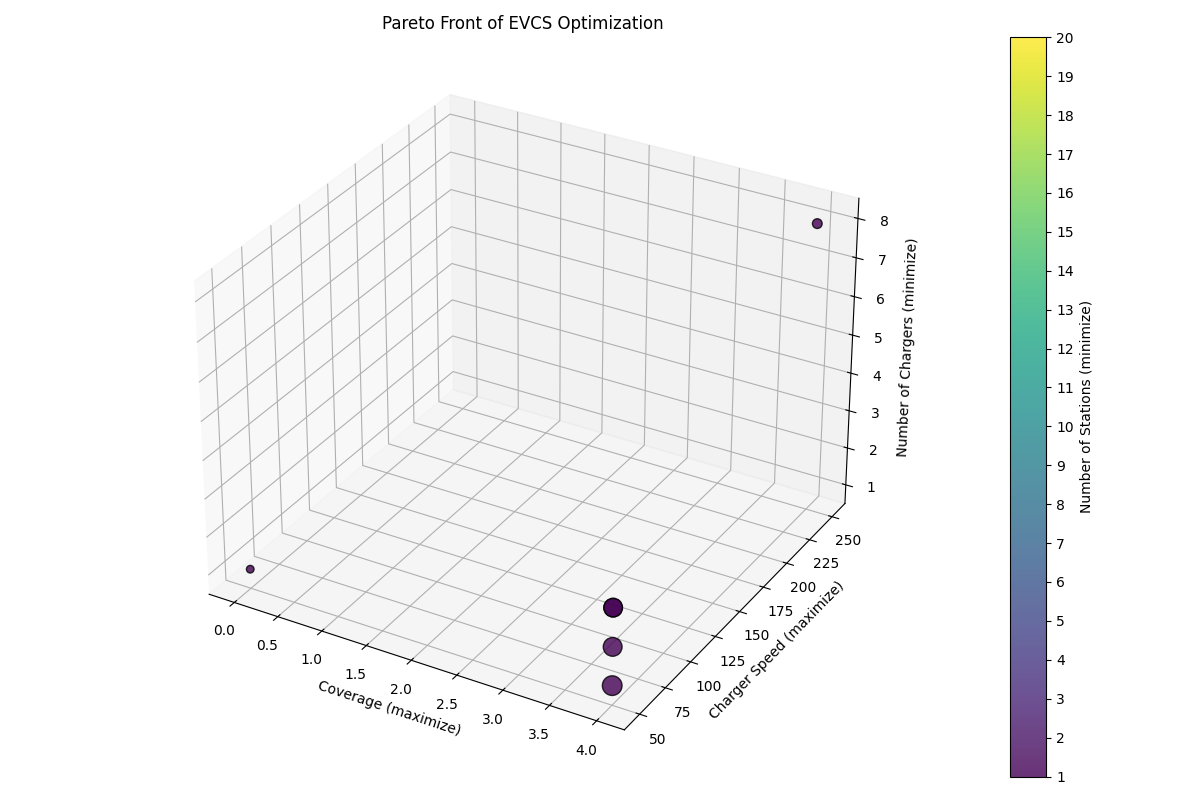
\includegraphics[width=0.8\textwidth]{../Figures/Pareto_Front.png}
    \caption{Pareto Front from NSGA-II Optimization}
    \label{fig:pareto-front}
\end{figure}

\subsection{Trade-off Analysis}

Table~\ref{tab:trade-off} presents four representative solutions from the Pareto front, each highlighting distinct trade-off configurations. These solutions illustrate how different balances between the objectives (coverage, charger speed, number of stations, and number of chargers) affect the overall performance. 

In addition, by analyzing these solutions, we can better understand how adjusting one objective impacts the others, helping to identify optimal configurations for the charging station network. This provides valuable into the relationship between the competing objectives and their influence on the final solution.

\begin{figure}[h]
    \centering
    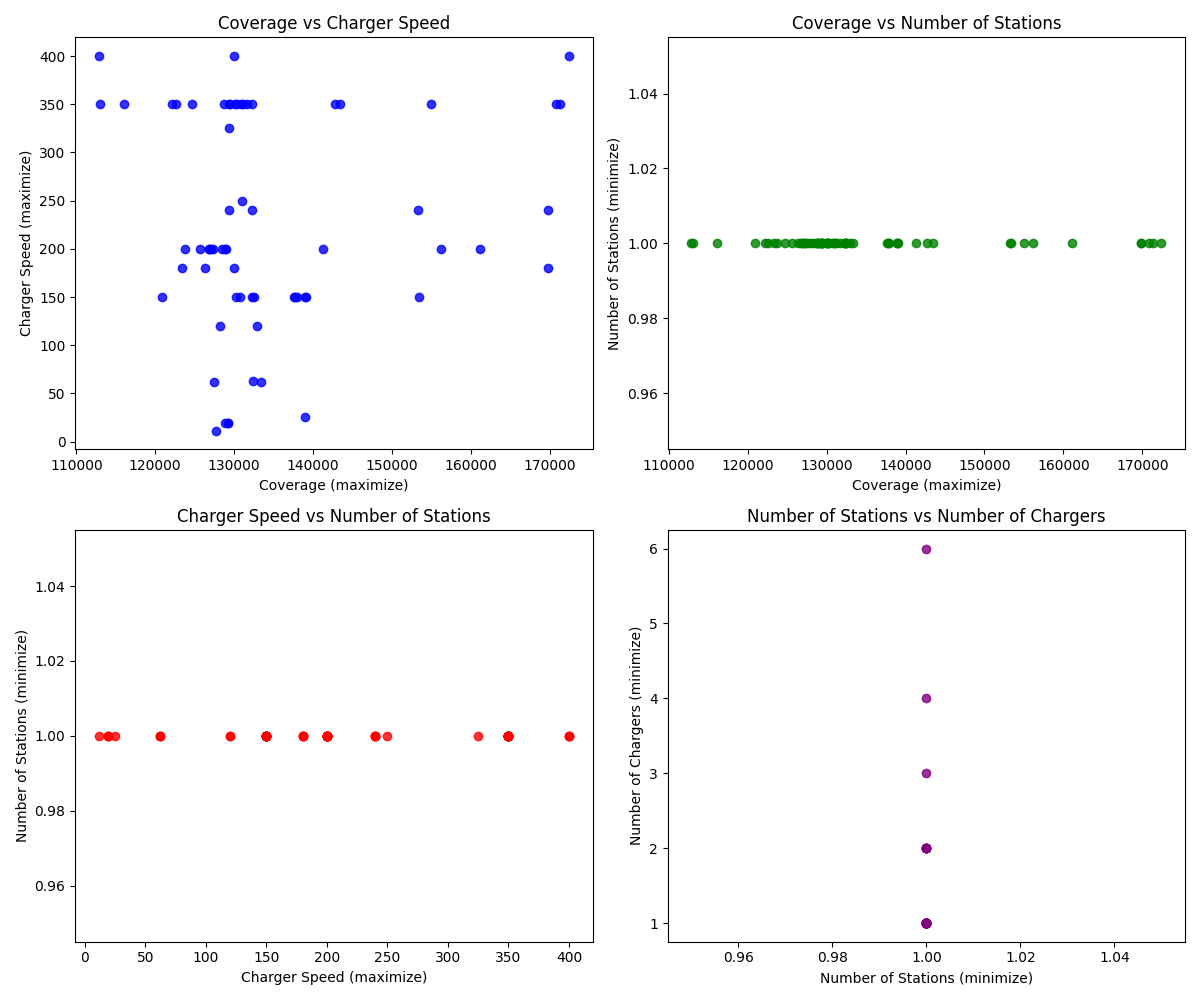
\includegraphics[width=0.8\textwidth]{../Figures/Trade_Off.png}
    \caption{Trade-Off from NSGA-II Optimization}
    \label{fig:trade-off}
\end{figure}